\documentclass[11pt,a4paper]{article}

\usepackage[utf8]{inputenc}
\usepackage[T1]{fontenc}
\usepackage[spanish]{babel}
\usepackage[margin=1.5cm, top=1.5cm, bottom=1.5cm]{geometry}
\usepackage{graphicx}
\graphicspath{{../../01_Propuesta/Logos/}{./}}
\usepackage{fancyhdr}
\usepackage{xcolor}
\usepackage[hidelinks]{hyperref}
\usepackage{booktabs}

\definecolor{verdeosc}{RGB}{26,107,60}
\definecolor{verdemid}{RGB}{46,139,87}

\setlength{\headheight}{35pt}
\pagestyle{fancy}
\fancyhf{}
\fancyhead[L]{%
  \begin{tabular*}{\textwidth}{@{\extracolsep{\fill}}ccc@{}}
    
\includegraphics[height=1.3cm]{logo_unisucre.png} &
    
\includegraphics[height=1.3cm]{logo_sicvec2026.png} &
    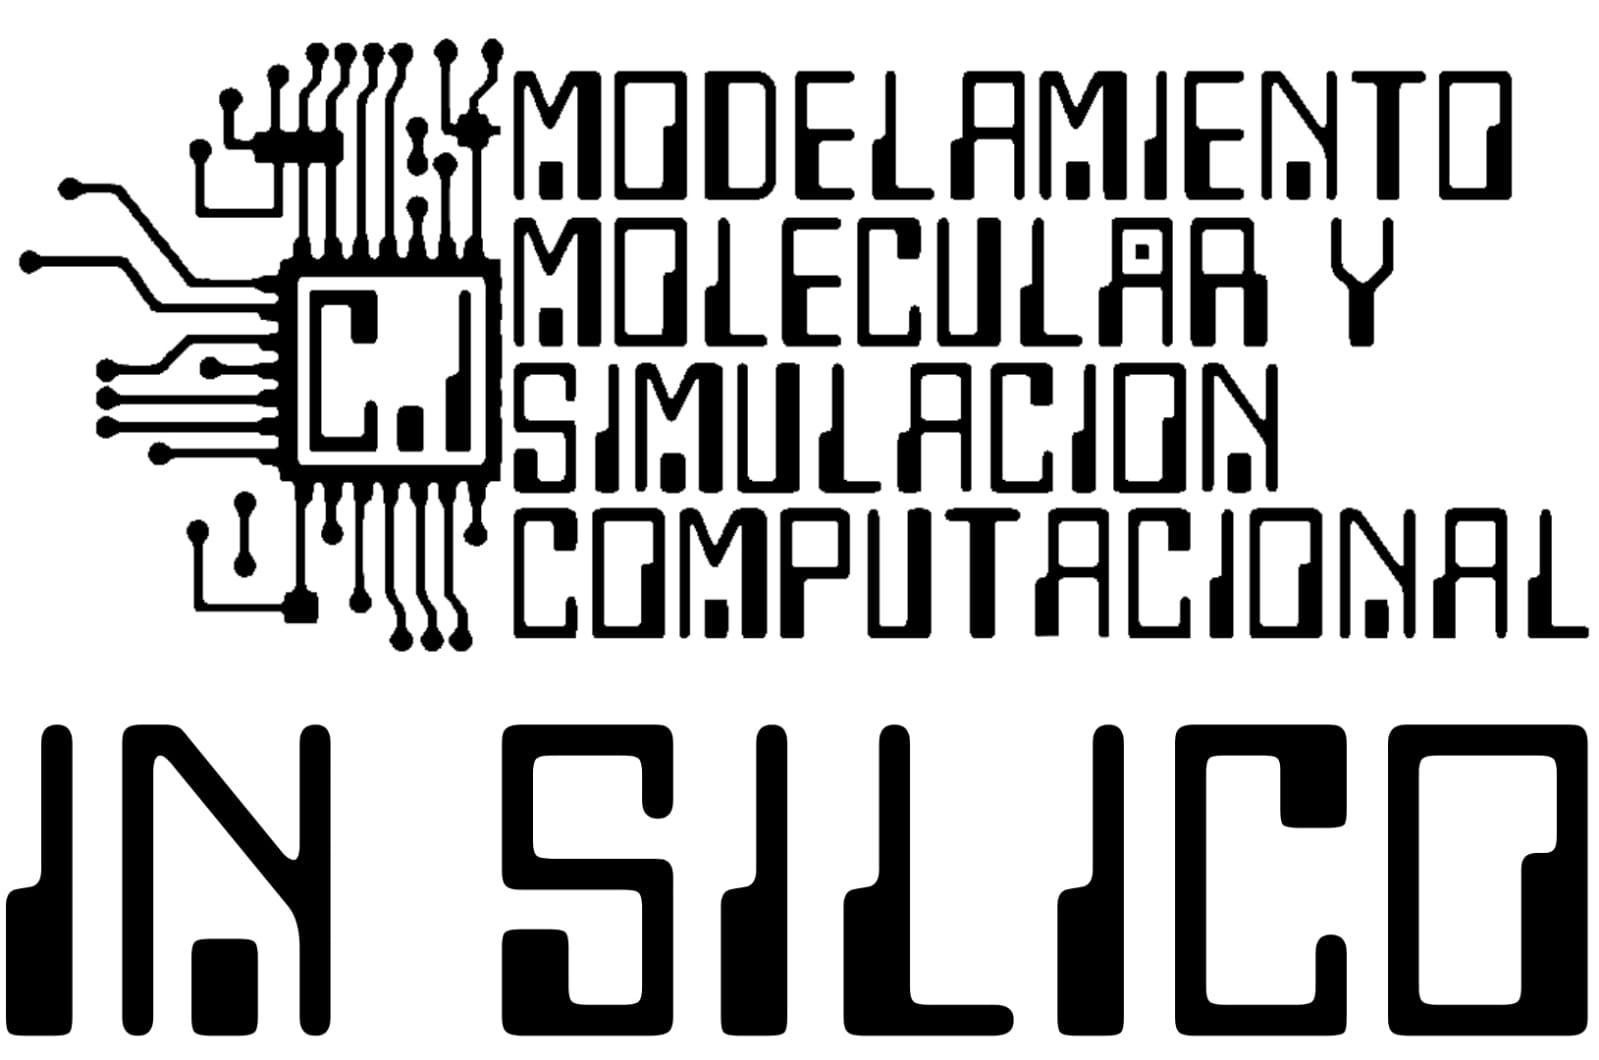
\includegraphics[height=1.3cm]{Logo_insilico.jpeg} \\
  \end{tabular*}%
}
\renewcommand{\headrulewidth}{1pt}
\renewcommand{\headrule}{\hbox to\headwidth{\color{verdeosc}\leaders\hrule height\headrulewidth\hfill}}

\begin{document}

\vspace{0.3cm}

\begin{center}
\textbf{\Large MUESTRA EMPRESARIAL Y PATROCINIO}

\textbf{\large SIMPOSIO INTERNACIONAL DE CIENCIA VERDE Y ECONOMÍA CIRCULAR}

\textbf{SICVEC 2026}

\textit{Propuesta de Participación Corporativa}
\end{center}

\vspace{0.4cm}

\section*{1. Oportunidad de Negocio}

El Simposio Internacional de Ciencia Verde y Economía Circular (SICVEC 2026) es una plataforma única para que empresas y organizaciones presenten sus soluciones, productos y servicios en sostenibilidad, química verde, energías renovables y tecnologías limpias a una audiencia altamente cualificada de investigadores, profesionales, tomadores de decisiones y emprendedores de Colombia, Latinoamérica e internacionalmente.

\vspace{0.2cm}

\section*{2. El Evento}

\begin{tabular}{ll}
\textbf{Fechas:} & 19 y 20 de octubre de 2026 (lunes y martes) \\
\textbf{Horario:} & 08:00 — 18:00 (ambos días) \\
\textbf{Lugar:} & Centro Comercial Guacarí, Sincelejo, Sucre, Colombia \\
\textbf{Modalidad:} & Híbrida (presencial + virtual) \\
\textbf{Audiencia:} & 120–150 asistentes presenciales + 100 cupos virtuales \\
\end{tabular}

\vspace{0.2cm}

\section*{3. Audiencia Objetivo}

\begin{itemize}\setlength{\itemsep}{0.1cm}
\item Investigadores y docentes en química verde, biotecnología y energías renovables
\item Profesionales en ingeniería ambiental, sostenibilidad e industria 4.0
\item Emprendedores y startups en tecnologías limpias
\item Tomadores de decisiones en empresas y gobiernos
\item Estudiantes de postgrado en disciplinas relacionadas
\item Medios de comunicación y periodismo científico
\end{itemize}

\vspace{0.2cm}

\section*{4. Participación Empresarial}

Ofrecemos un modelo flexible de participación corporativa mediante aporte en \textbf{efectivo o en especie}, sin restricción de montos predeterminados. Cada empresa define su nivel de contribución según sus capacidades y objetivos.

\subsection*{Beneficios de Participación}

\begin{itemize}\setlength{\itemsep}{0.08cm}
\item Stand de exhibición con mesa y sillas
\item Logo y nombre en comunicaciones del evento
\item Mención en materiales de difusión y promoción
\item Material promocional en carpetas de asistentes
\item Networking con investigadores, profesionales y emprendedores
\item Certificación de participación corporativa
\end{itemize}

\subsection*{Formas de Aporte}

\begin{itemize}\setlength{\itemsep}{0.08cm}
\item \textbf{Aporte en Efectivo:} Monto flexible a negociar (USD, COP u otra moneda)
\item \textbf{Aporte en Especie:} Productos, servicios, equipamiento, refrigerios, materiales promocionales u otros recursos que agreguen valor al evento
\item \textbf{Combinado:} Mezcla de efectivo y aporte en especie
\end{itemize}

\vspace{0.2cm}

\section*{5. Beneficios Adicionales}

\begin{itemize}\setlength{\itemsep}{0.08cm}
\item \textbf{Visibilidad Multi-canal:} Promoción en redes sociales, sitio web, email marketing (5.000+ contactos)
\item \textbf{Cobertura Mediática:} Transmisión en vivo, grabación y memorias ISBN con presencia corporativa
\item \textbf{Networking Premium:} Acceso a conferencistas invitados, investigadores y empresarios
\item \textbf{Certificación:} Reconocimiento formal de participación corporativa
\item \textbf{Alianzas Futuras:} Presentación ante red de investigadores activos en sostenibilidad e innovación
\end{itemize}

\vspace{0.2cm}

\section*{6. Logística de Stands}

\begin{itemize}\setlength{\itemsep}{0.08cm}
\item Stands ubicados en sala de exhibiciones del Centro Comercial Guacarí
\item Acceso a servicios básicos (electricidad, WiFi, agua)
\item Montaje: 17–19 octubre (día previo al evento)
\item Desmontaje: 20 octubre (después de las 18:00)
\item Seguridad y supervisión durante el evento
\item Parqueo para vehículos de carga durante montaje/desmontaje
\end{itemize}

\vspace{0.2cm}

\section*{7. Ejes Temáticos — Oportunidades Sectoriales}

\begin{itemize}\setlength{\itemsep}{0.08cm}
\item \textbf{Química Verde y Procesos Sostenibles:} Empresas de químicos eco-amigables, bioprocesos
\item \textbf{Tecnologías Verdes y Energías Renovables:} Solar, eólica, hidrógeno, almacenamiento
\item \textbf{Biotecnología Sostenible:} Bioproductos, biocombustibles, bioremediación
\item \textbf{Economía Circular:} Gestión de residuos, reciclaje, recuperación de recursos
\item \textbf{Sostenibilidad en Cadenas de Suministro:} Logística verde, trazabilidad digital
\end{itemize}

\vspace{0.2cm}

\section*{8. Próximos Pasos}

\begin{enumerate}\setlength{\itemsep}{0.1cm}
\item Contactar al coordinador para confirmar interés
\item Completar formulario de solicitud y enviar logo/materiales
\item Confirmar paquete y procesar pago (antes de 30 septiembre para confirmación)
\item Recibir confirmación y detalles logísticos finales
\item Participar en evento y maximizar impacto corporativo
\end{enumerate}

\vspace{0.3cm}

\section*{9. Contacto}

\textbf{Coordinación de Patrocinio y Exhibición:}

Selena Arias Avila \\
Coordinadora Administrativa, SICVEC 2026 \\
Grupo de Investigación IN SILICO \\
Universidad de Sucre, Colombia \\
Email: \href{mailto:SelenaAriasAvila07@gmail.com}{SelenaAriasAvila07@gmail.com} \\
Teléfono: \href{tel:+573042541353}{(+57) 3042541353}

\vspace{0.3cm}

\noindent
\rule{\textwidth}{0.5pt}

\vspace{0.2cm}

\noindent
\textit{\small SICVEC 2026 es una iniciativa de ciencia e innovación en sostenibilidad. Contribuye a los ODS: 12 (Consumo responsable), 13 (Acción climática), 15 (Vida terrestre), 17 (Alianzas).}

\end{document}
